\section{Air Quality}
\subsection{Air pollution}
Air pollution can be defined as a group of chemicals present in the atmosphere harmful for humans, animals or vegetation. They are mainly caused by human activities, such as transport, industry, or agriculture. But they can also be influenced by other natural sources. Understanding air pollution is important because many health consequences are brought from high pollution levels. 
\begin{figure}[h]
  \centering
  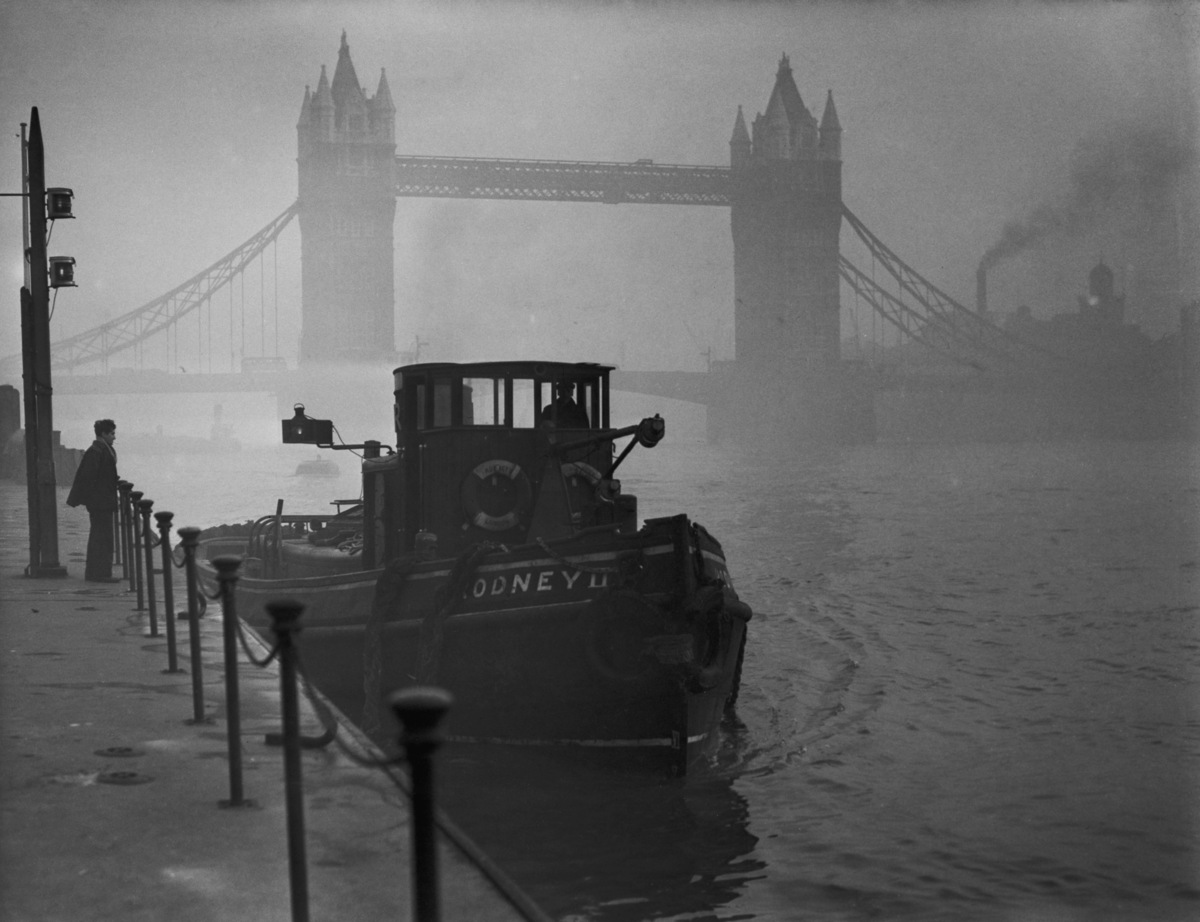
\includegraphics[scale=.8]{images/great_smog.jpg}
  \caption[Great smog of 1952]{Great smog of 1952 \cite{ElliotWagland2013}}
  \label{fig:interaction_design}
\end{figure}

One historic event which caused huge consequences is known as the the great smog of 1952. Thousands of persons died in Greater London due to  breathing for various days a highly contaminated atmosphere and many others became ill or experienced retarded symptoms \cite{Bell2008}. The fog originated from coil burning, vehicle exhaust and other atmospheric factors. Although many human activities introducing pollution particles have changed since then, it became evident the immediate and retarded health impact of pollution particles.

Pollution chemicals can be categorized into gaseous pollutants, persistent organic pollutants, heavy metals and particulate matter. They change on chemical composition, emission sources and impact on health. Gaseous pollutants are sulfur dioxide (\SOTWO), nitrogen oxides (\NOX), carbon monoxide (CO), ozone (\OTHREE) and volatile organic compounds. The principal source of this gas pollutants is combustion. 

Nitrogen oxides (\NOX) is a general term that includes nitric oxide (NO) and nitrogen oxide \NOTWO. NO and \NOTWO come from combustion of fossil fuels such as coal and natural gas.

Particulate matter (PM) is a mixture of solid and liquid particles including sulfate, nitrates, ammonia, sodium chloride, black carbon, mineral dust and water. The sources of PM are mainly vehicle, industrial and domestic exhaust, but they also include forest fires and cigarette smoke. PM are categorized according their diameter size measured in microns (μm, 1×10−6 of a metre). Particles smaller than 10 microns (\PMTEN) are known as coarse particles, smaller particles with a size of up to 2.5  and 1 microns are known as fine and ultra-fine particles respectively. They are differentiated in sizes because it dictates their aerodynamic properties, that is, how they are transported into the air, as well as how far they can get into the respiratory system.

Carbon Monoxide

Ozone 

Air quality is also affected by pollution mixture in further complex chemical structures and by temperature and humidity conditions . \NOTWO, PM and O\textsubscript{2}  pollutants get transformed by atmospheric processes making complex to evaluate their individual impact. As an example, ground level ozone is produced when sunlight interacts with \NOTWO and volatile organic compounds. Furthermore, \NOTWO and other nitrogen oxides also contribute to PM generation, making \NOX a particularly concerning pollutant.


\subsection{Air pollution Health effects}

 The health effects of NO\textsubscript{x} are irritating the lungs and increasing susceptibility to respiratory infections like influenza[].
 According to the World Health Organization, PM is the most harmful pollutant because it can pass through the nose and throat and enter the lungs. PM 
 
Exposure to PM is associated with risk of cardiovascular disease \cite{Polichetti2009}

Chronic exposure to ozone and certain heavy metals reduces lung function \cite{Kampa2008}

\subsection{Air quality data dissemination}
Providing open air quality data to the general public aimed to have informed and aware citizens that could take part into more sustainable and environmental choices. "Yet, what was lacking (and it still is), is a model for effective communicating of environmental information to the public" \cite{Thinh2007}. Terms like assessment, limit values, target values and concentration, among others are commonly used by air quality data publishers to describe the current or forecasted quality status; however, there is not a common ground on how the air quality information should be disseminated to the general public in a way it is understood immediately and intuitively. 

In general it is complex to categorize and establish measures for the different components of air pollution due their homogeneous nature and the chemical reactions that occur in between them. Measurement methods and units vary from institution to institution and regulation standards can be specific for each country, which may rise ambiguity. Furthermore, much of the available data is represented in a plain tabular format, including various information for individual pollutants, as exemplified in table \ref{tab:pollution_tabular_data}. This table was extracted from the  Department for Environment Food and Rural Affairs (DEFRA) website \cite{DepartmentforEnvironmenta}, it shows measures related to the air quality from a sensing station located in Deaconess Garden in the south of Edinburgh. At first sight it table arises some questions for the novice on air-quality trying to crack the data. Firstly, the pollution codes such as PM2.5, PM10, NO2, NOXasNO2 and their subtle differences should be understood. Secondly, some measurement units are tagged with the monitoring method used to extract the information, like the TEOM FDMS \footnote{Which indicates that the sensing methods were Tapered Element Oscillating Microbalance and Filter Dynamics Measurement System \cite{Quality2005}} tag. And lastly, it is difficult to know which measurements are of more interest given a person specific circumstances. As stated by Brimblecombe and Schuepbach \cite{P.Brimblecombe2008}, "many people complain that the information is unintelligible, while some have even seen it as an attempt of government to blind the public with science", it is clearly difficult to understand the meaning of the terms and values that are used to represent air quality data to the general public. 
\begin{table}[ht]
\centering
\begin{adjustbox}{width=1.2\textwidth,center=\textwidth}
\begin{tabular}{rlrrrrrrr}
  \hline
 Pollutant & Date & Time & Measurement & Unit & Period & Comment  \\ \hline
    Ozone (O3) & 20/07/2016 & 07:00 & 63.06412 & µg/m3 & Hourly & - \\
    Nitric oxide (NO) & 20/07/2016 & 07:00 & 2.61933 & µg/m3 & Hourly & - \\
    Nitrogen dioxide (NO2) & 20/07/2016 & 07:00 & 27.34875 & µg/m3 & Hourly & - \\
    Nitrogen oxides as nitrogen dioxide (NOXasNO2) & 20/07/2016 & 07:00 & 31.36500 & µg/m3 & Hourly & - \\
	Sulphur dioxide (SO2) & 20/07/2016 & 07:00 & 14.63495 & µg/m3 & Hourly & - \\
	Carbon monoxide (CO) & 20/07/2016 & 07:00 & 0.081494 & mg/m3 & Hourly & - \\
	PM10 particulate matter (Hourly measured) (PM10) & 18/07/2016 & 15:00 & 10.900 & µg/m3 (TEOM FDMS) & Hourly & - No current data. \\
	Non-volatile PM10 (Hourly measured) (Non-volatile PM10) & 19/07/2016 & 07:00 & 26.700 & µg/m3 (TEOM FDMS) & Hourly & - No current data. \\
	Volatile PM10 (Hourly measured) (Volatile PM10) & 19/07/2016 & 07:00 & 5.500 & µg/m3 (TEOM FDMS) & Hourly & - No current data. \\
	PM2.5 particulate matter (Hourly measured) (PM2.5) & 18/07/2016 & 15:00 & 4.300 & µg/m3 (TEOM FDMS) & Hourly & - No current data. \\
	Non-volatile PM2.5 (Hourly measured) (Non-volatile PM2.5) & 19/07/2016 & 07:00 & 16.300 & µg/m3 (TEOM FDMS) & Hourly & - No current data. \\
	Volatile PM2.5 (Hourly measured) (Volatile PM2.5) & 19/07/2016 & 07:00 & 5.000 & µg/m3 (TEOM FDMS) & Hourly & - No current data. \\
	Modelled Wind Direction (Dir) & 19/07/2016 & 24:00 & 50.6 & \degree & Hourly & - No current data. \\
	Modelled Wind Speed (Speed) & 19/07/2016 & 24:00 & 6.2 & m/s & Hourly & - No current data. \\
	Modelled Temperature (Temp) & 19/07/2016 & 24:00 & 14.6 & °C & Hourly & - No current data. \\
	PM10 Ambient Temperature (AT10) & 19/07/2016 & 07:00 & 19.4 & °C & Hourly & - No current data. \\
	PM10 Ambient pressure measured (AP10) & 19/07/2016 & 07:00 & 989.0 & mb & Hourly & - No current data. \\
	PM2.5 Ambient Temperature (AT25 ) & 19/07/2016 & 07:00 & 17.5 & °C & Hourly & - No current data. \\
	PM2.5 Ambient Preasure (AP25) & 19/07/2016 & 07:00 & 988.0 & mb & Hourly & - No current data. \\
   \hline
\end{tabular}
\end{adjustbox}
\caption{Air quality tabular data representation. \cite{DepartmentforEnvironment}}
\label{tab:pollution_tabular_data}
\end{table} 

\subsection{Air quality Index}
In order to understand the correlation between air quality data and its effects in human health, the \ac{COMEAP} developed the air quality index based on health evidence. It is used to communicate real time air quality levels and their short-term health effects for five selected harmful pollutants: particulate matter (\PMTEN), ozone (\OTHREE), sulphur dioxide (\SOTWO), carbon monoxide (CO) and nitrogen dioxide (\NOTWO). The choice 
There are four bands: Low, Moderate, High and very high levels. 

\begin{figure}[H]
\begin{adjustbox}{width=1\textwidth,center=\textwidth}
  \centering
  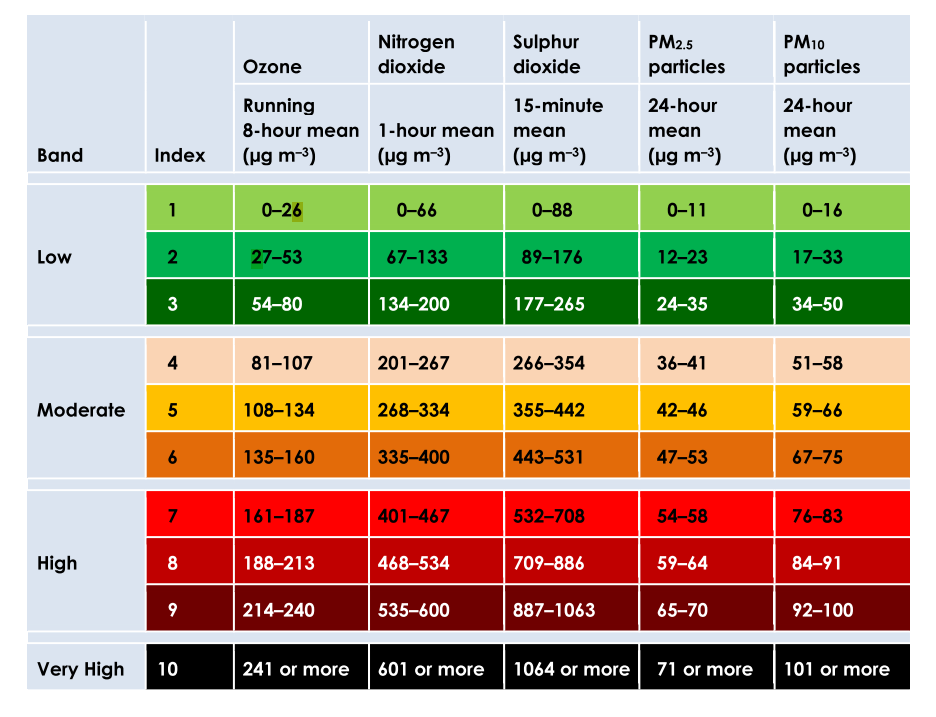
\includegraphics[scale=.8]{images/air_quality_index.png}
  \label{fig:air_quality_index}
\end{adjustbox}
  \caption[The COMEAP air quality index]{The COMEAP air quality index \cite{HealthProtectionAgencyfortheCommitteeontheMedicalEffectsofAirPollutants2011}}
\end{figure}

There is this health advice accompanying the health index.

\begin{figure}[H]
\begin{adjustbox}{width=1\textwidth,center=\textwidth}
  \centering
  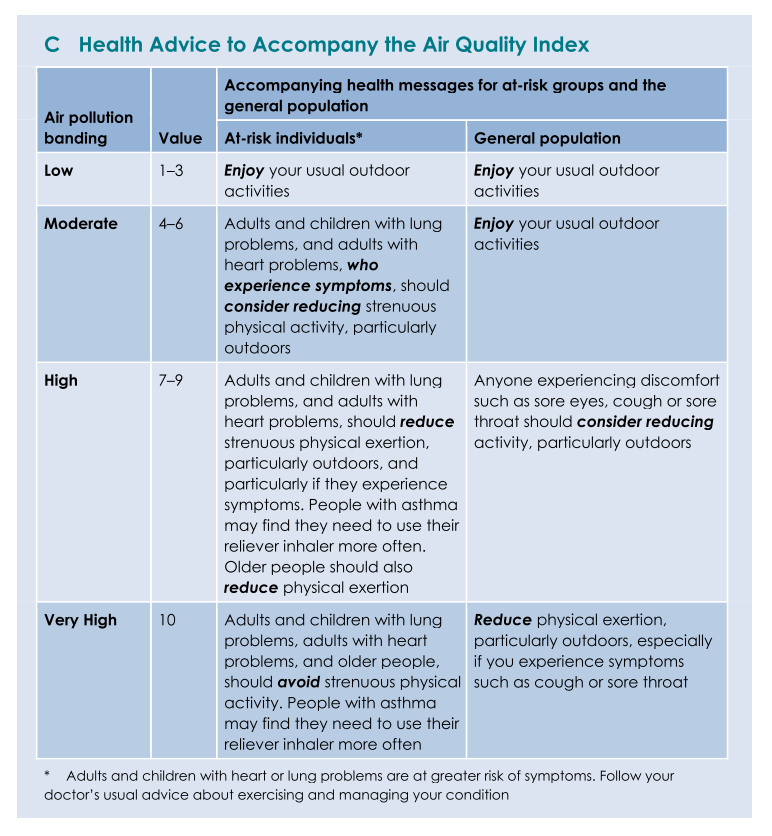
\includegraphics[scale=.8]{images/air_quality_health_advice.png}
  \label{fig:air_quality_health_advice}
\end{adjustbox}
  \caption[Air quality health advice]{Air quality health advice \cite{HealthProtectionAgencyfortheCommitteeontheMedicalEffectsofAirPollutants2011}}
\end{figure}

\subsection{Air quality policies}
How air quality policies differ around the world, and why this might be a problem.

\subsection{Air quality sensors}

\begin{itemize}

\item Fixed sensors

\item Portable sensors

\item Participatory sensors

Some projects include users as 'human sensors' by reading the perceptions about the users towards air quality in certain locations with a mobile application (REF), and online questionnaires (REF). This method aims to get more fine-grained information about air quality and engage the citizens in the pollution problem and its solution. However, this readings lack of credibility and it is hard to use them for real world applications.

\end{itemize}



